\subsection{Recoverable Distributor}

In many distributed systems, there is a need to share a state across distributed
components. Maintaining consistency in the shared state amongst the components
and providing a fault tolerant system requires special attention. The
Recoverable Distributor pattern provides means for a group of distributed
objects to share a common state and addresses performance, fault tolerance, and
recovery issues \cite{RD1}. 

The Recoverable Distributor pattern is described in \cite{RD1} and \cite{RD2} to
maintain one global state and many private states for each distributed component
involved (see Figure \ref{fig:rd}. This private view is used locally, which
allows for higher performance than continuously depending on and requesting the
global state. These private, or local, states are kept consistent with the
global state by the \texttt{ConcreteGlobalStateManager}. The
\texttt{ConcreteGlobalStateManager} keeps track of the
\texttt{LocalStateManager}s, each of which is native to one of the distributed
components. The \texttt{LocalStateManager} is an interface that defines how the
\texttt{GlobalStateManager} is informed of any local changes in state. The
\texttt{ConcreteLocalStateManager} implements this interface and also stores the
local state. Any changes to this state are propagated to the
\texttt{ConcreteGlobalStateManager}. The \texttt{ConcreteGlobalStateManager}
utilizes the \texttt{add(LocalStateManager} and
\texttt{delete(LocalStateManager)} methods of its interface
\texttt{GlobalStateManager} to upkeep its list of participating
\texttt{LocalStateManager}s. This interface also defines an interface to notify
all of the enlisted \texttt{LocalStateManager}s of any changes to the global
state. The \texttt{ConcreteGlobalStateManager} contains and maintains the global
state, allowing for the returning and updating of the its current state. These
collaborators jointly maintain consistency among the global and local states and
provide recovery methods in cause of failure.

\begin{figure}
\begin{center}
  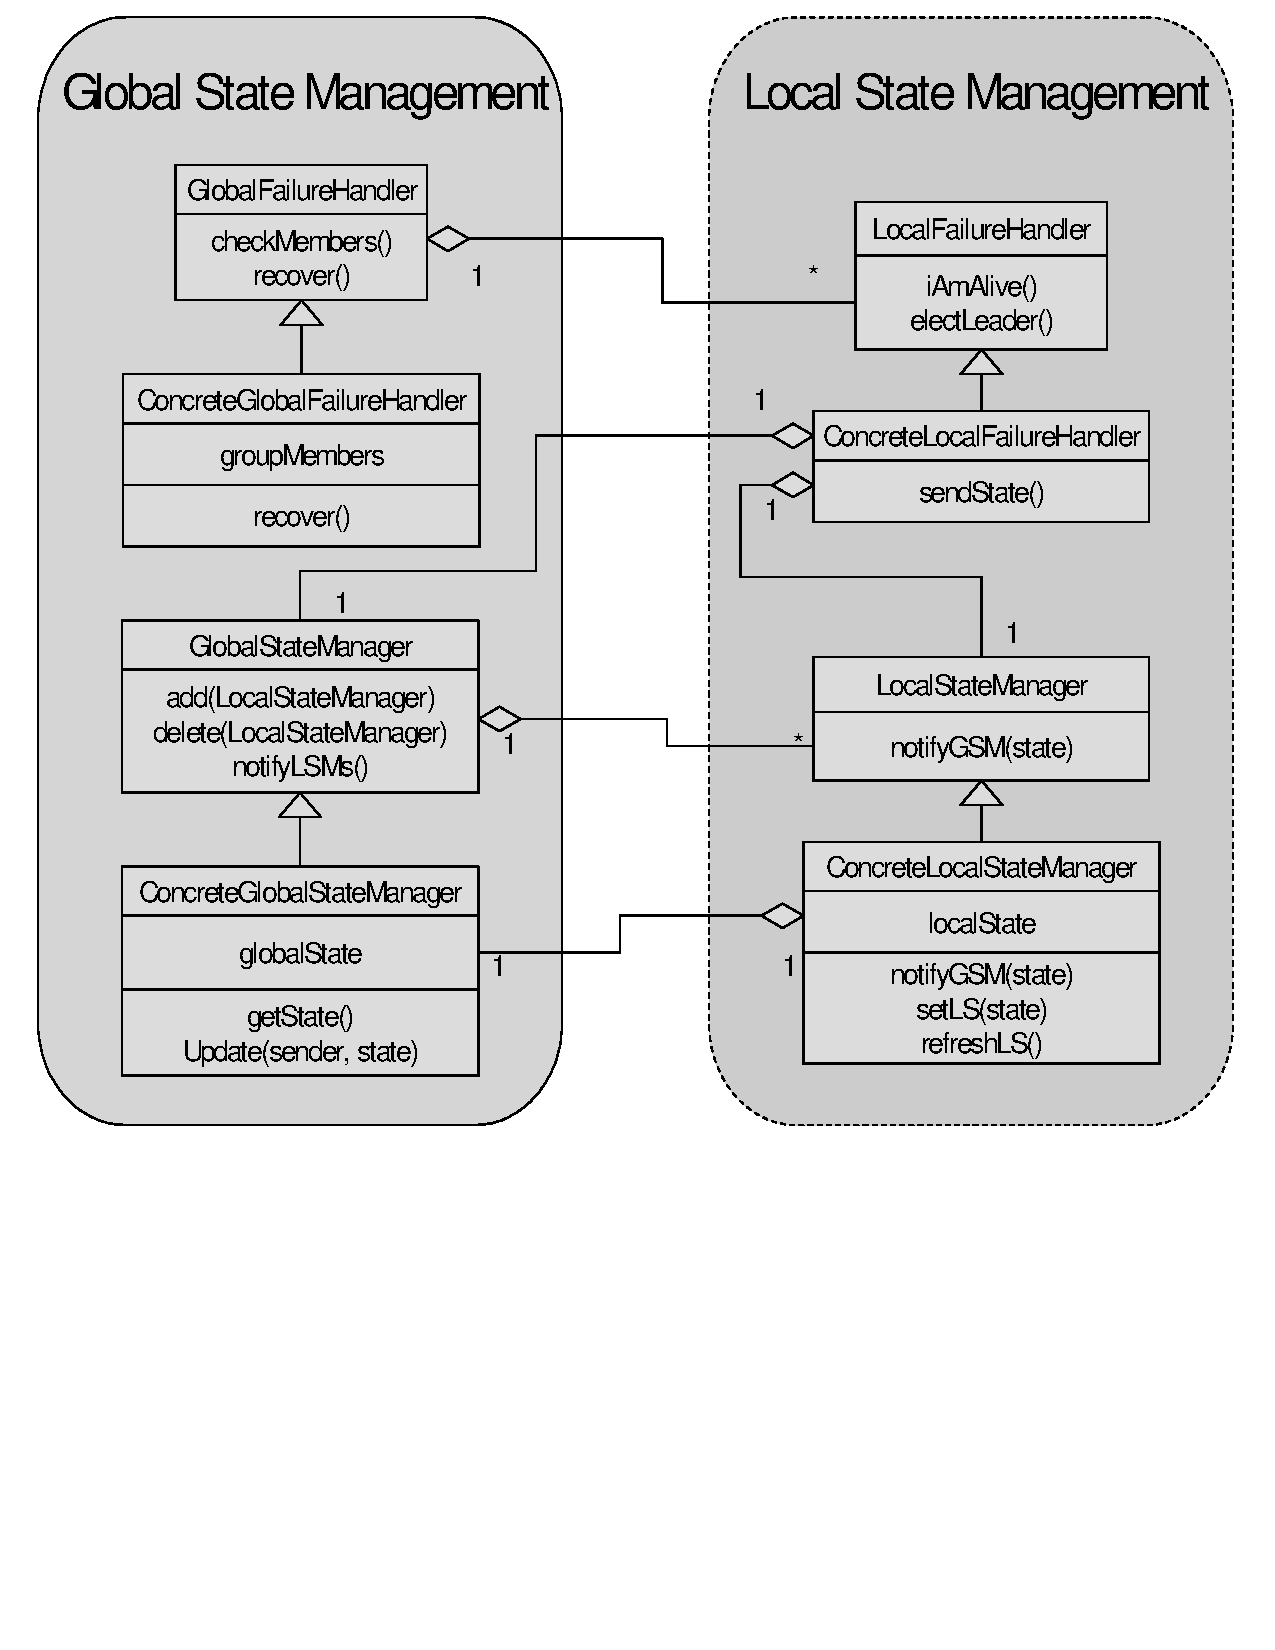
\includegraphics[width=0.9\textwidth]{./images/recoverableDistributor}
  \caption{Recoverable Distributor UML Diagram}
  \label{fig:rd}
\end{center}
\end{figure}

The Recoverable Distributor pattern also addresses recovery issues when one of
the distributed components fail. A \texttt{ConcreteGlobalFailureHandler}
maintains a list of subscribed members. It implements the
\texttt{GlobalFailureHandler} interface, which defines methods to detect the
failure of nodes and to recover from these failures. the
\texttt{ConcreteGlobalFailureHandler} will periodically poll its members through
each member's \texttt{LocalFailureHandler} to check that they are still live. If
a \texttt{LocalFailureHandler} does not respond, the
\texttt{GlobalFailureHandler} assumes that it and its associated
\texttt{LocalStateManager} has failed. In the event of this failure, the
\texttt{GlobalFailureHandler} will recognize its need to recover. Failure of a
\texttt{LocalStateManager} introduces the possibility of inconsistency amongst
distributed nodes. Thus, the \texttt{GlobalFailureHandler} starts reconstruction
of its global state through the remaining live local states.

\subsubsection{Tomcat cluster and session replication}

Tomcat 5's cluster and session replication techniques are described in
\cite{Tomcat} and \cite{Tomcat2}. The main element in Tomcat's cluster and
session replication implementation is the cluster and its nodes. The
\texttt{SimpleTcpCluster} is a cluster element. The first element that joins the
cluster creates the \texttt{ClusterManager} that manages the replicated content
and the members in the cluster. The \texttt{ClusterManager} replicates the
session data on all of the members of the cluster. Tomcat provides two
replication algorithms, one that replicates the entire session every time and
one that only replicates changes in the session. Since Coursebook's sessions
will have minimal attributes in each session, replicating the entire session
does not entail the performance hits of other more complex requests and
sessions. For simplicity, we would choose to replicate the entire session for
each request for Coursebook. This technique uses the
\texttt{SimpleTcpReplicationManager}, which implements the
\texttt{ClusterManager} interface. Before the response to a request is returned
to the user, the \texttt{ReplicationValve} determines if the request needs to be
replicated. In other words, the \texttt{ReplicationValve} determines if the
session has been changed and the replicated state needs to be updated. The
\texttt{ReplicationValve} initiates the replication by notifying the manager of
the request completion and if the state was updated.

\begin{figure}
\begin{center}
  \centering
  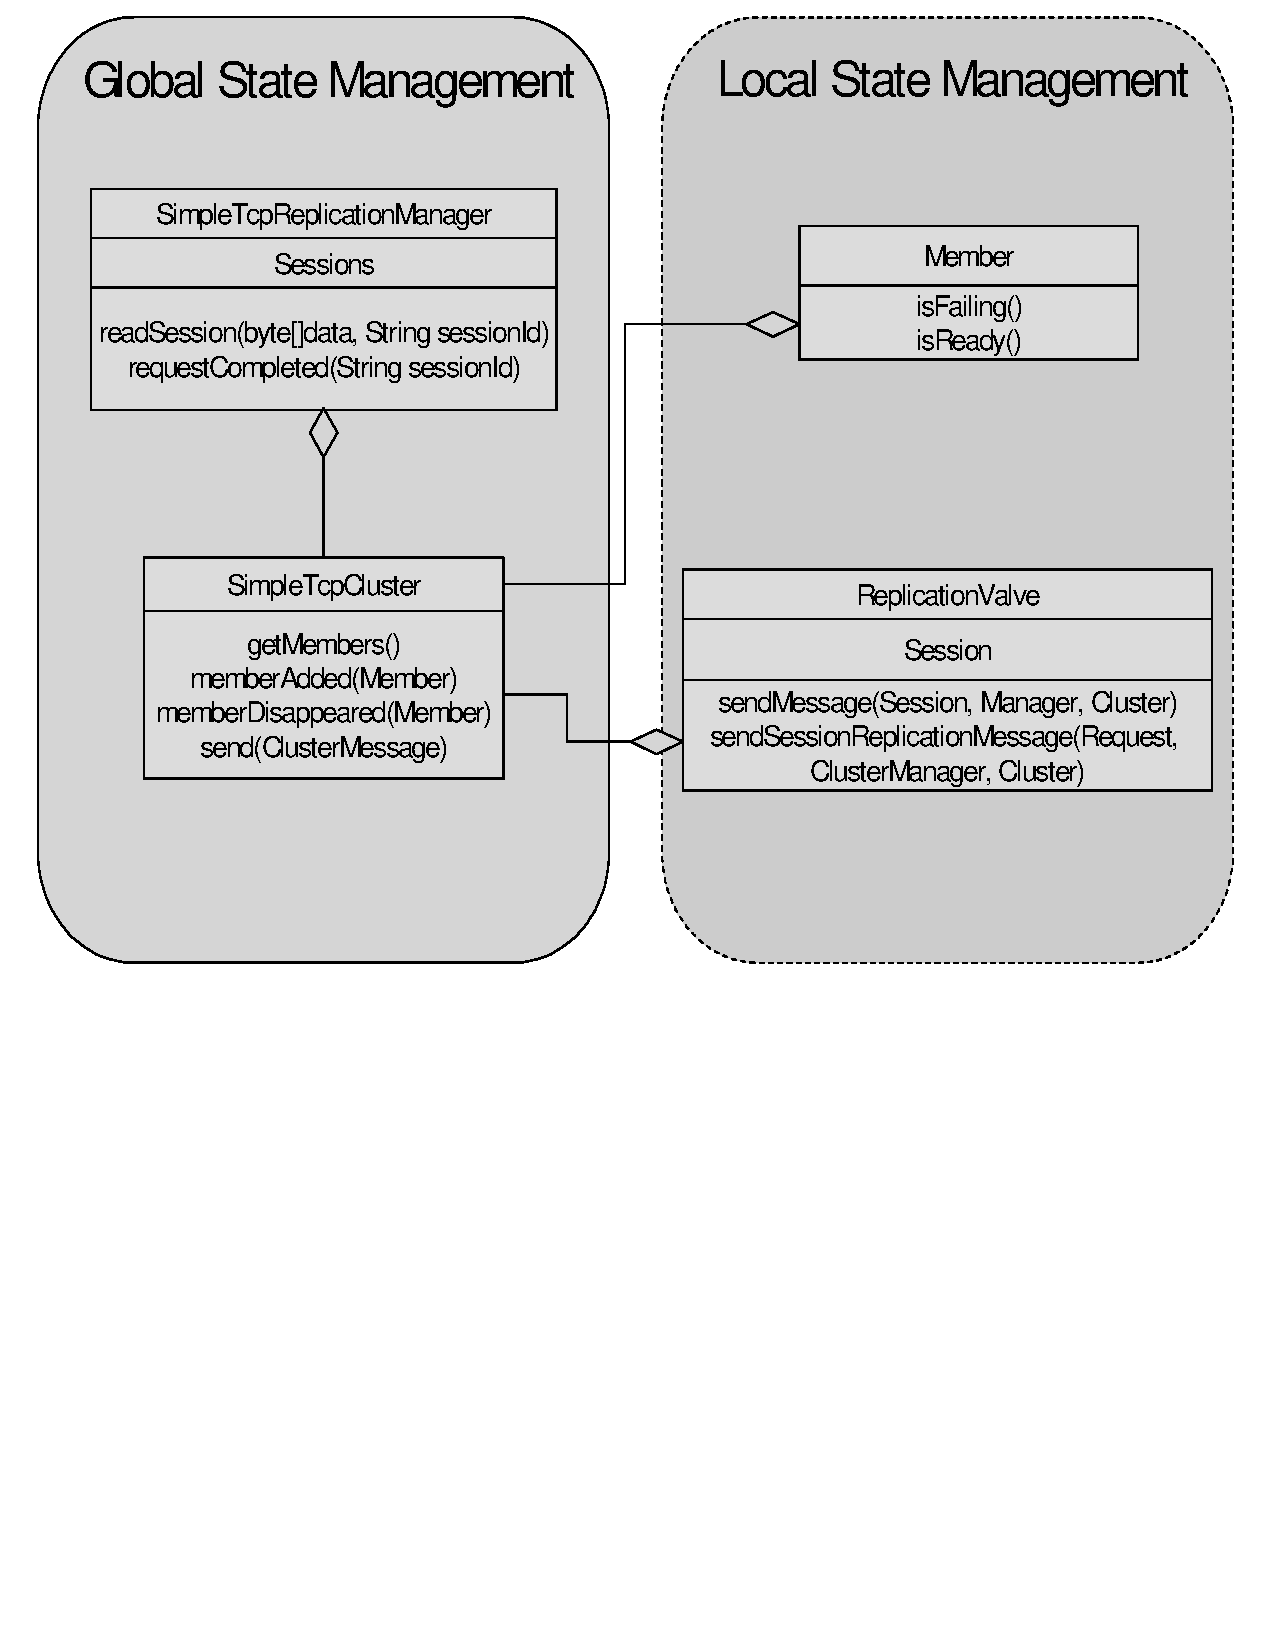
\includegraphics[width=0.9\textwidth]{./images/tomcatRecoverableDistributor}
  \caption{Tomcat's Use of Recoverable Distributor}
  \label{fig:tomcat}
\end{center}
\end{figure}

Embedded in Tomcat's session replication design is the RecoverableDistributor
design pattern, as shown in Figure \ref{fig:tomcatRecoverableDistributor}.
Tomcat's implementation is at a more complicated level. Rather than just dealing
with one state that is common amongst all the distributed nodes of the system,
Tomcat handles many different sessions that are replicated on all the nodes in
the cluster. The \texttt{SimpleTcpReplicationManager} represents the
\texttt{GlobalStateManager} that maintains and updates the global state of a
particular session. The \texttt{ReplicationValve} acts as a 
\texttt{LocalStateManager} that determines when a local state has changed and
propogates those changes to the manager, which eventually updates all the other
nodes in the cluster. This design is fault tolerant when one of the nodes in the
cluster fails; in such a case, the replicated session residing on another node
allows that node to handle any further requests in that session.

The future of Coursebook is designed to use Tomcat's clustering and session
replication techniques, and thus the RecoverableDistributor pattern. There are
several advantages in replicating sessions across nodes in a cluster. The first
of these advantages is performance \cite{Tomcat}. Load balancing across the
nodes in a cluster will result in a faster perceived response time for the user.
Also, storing the session locally removes the overhead of requesting the common
global state across nodes. Secondly, the reliability and fault tolerance of the
Coursebook is raised through the replication of the sessions across the cluster
nodes \cite{Tomcat}. The failure of any node can be recovered by utilizing the
replicated session on another node in the cluster. These advantages are the core
benefits of using the Recoverable Distributor pattern. Thus, further work on the
design and implementation of Coursebook will include Tomcat's use of the 
Recoverable Distributor pattern.
